\newpage
\subsection{QuizziPedia::Front-End::Services}
\begin{figure}
	\centering
	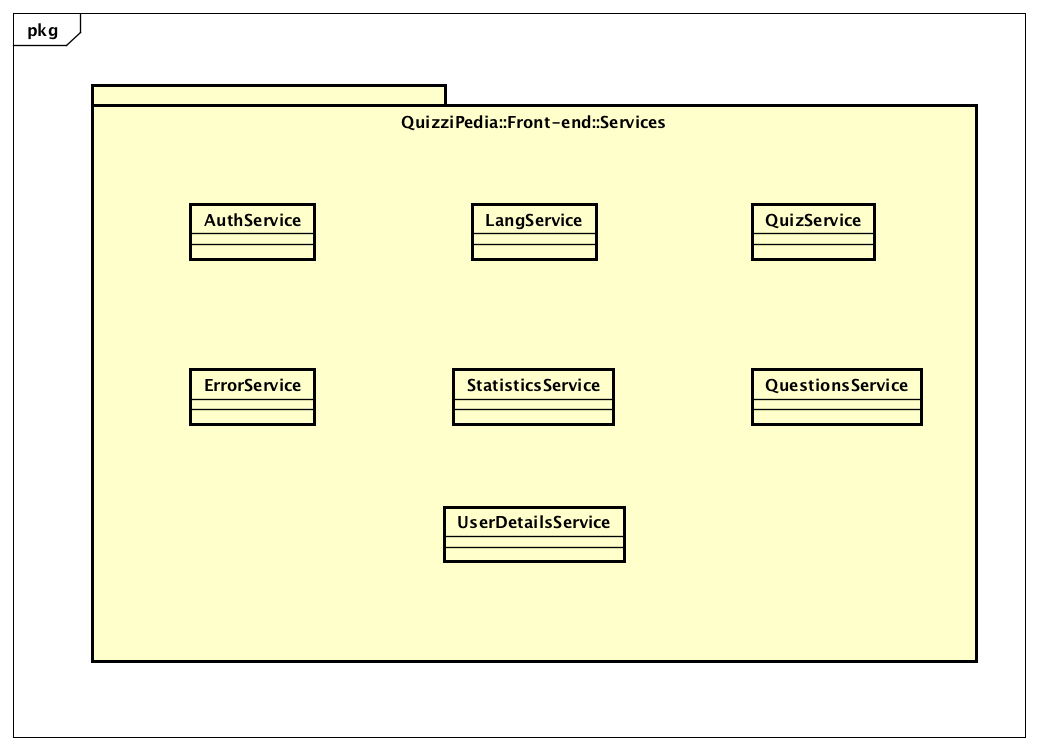
\includegraphics[scale=0.45]{UML/Package/QuizziPedia_Front-End_Services.png}
	\caption{QuizziPedia::Front-End::Services}
\end{figure}
\subsubsection{Informazioni generali}
\begin{itemize}
	\item \textbf{Descrizione}: package che contiene le classi individuate che permettono la comunicazione del lato front-end con il lato back-end;
	\item \textbf{Padre:} \texttt{Front-End};
	\item \textbf{Interazione con altri componenti:}
	\begin{itemize}
		\item \texttt{Models} - package che contiene le classi model individuate;
		\item \texttt{Controllers} - package che contiene le classi controller individuate.
	\end{itemize} 
\end{itemize}
\subsubsection{Classi}

\paragraph{QuizziPedia::Front-End::Services::AuthService}
\begin{figure}
	\centering
	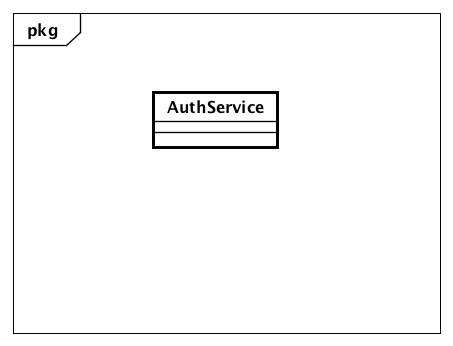
\includegraphics[scale=0.45]{UML/Classi/Front-End/QuizziPedia_Front-end_Services_ AuthService.png}
	\caption{QuizziPedia::Front-End::Services::AuthService}
\end{figure}
\begin{itemize}
	\item \textbf{Descrizione}: questa classe permette di gestire la registrazione e l'autenticazione di un utente;
	\item \textbf{Utilizzo}: fornisce le funzionalità di registrazione e autenticazione ai controllers. Controlla che i dati inseriti dall'utente siano presenti nel \textit{Database\ped{G}} in caso di autenticazione. Presenta anche le funzionalità per la gestione del reset della password;
	\item \textbf{Relazione con altre classi:}
	\begin{itemize}
		\item \textit{IN} \texttt{LoginController}: questa classe gestisce la logica alla base della pagina di autenticazione;
		\item \textit{IN} \texttt{PasswordForgotController}: questa classe gestisce la logica alla base del reset della password;
		\item \textit{IN} \texttt{SignUpController}: questa classe gestisce la logica alla base della registrazione di un nuovo utente.
	\end{itemize}
	\item \textbf{Attributi:}
	\begin{itemize}
		\item 
	\end{itemize}
	\item \textbf{Metodi:}
	\begin{itemize}
		\item 
	\end{itemize}
\end{itemize}

\paragraph{QuizziPedia::Front-End::Services::LangService}
\begin{figure}
	\centering
	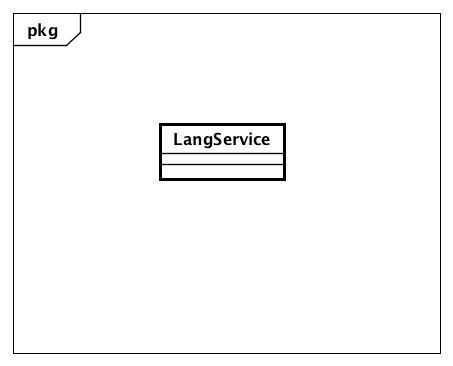
\includegraphics[scale=0.45]{UML/Classi/Front-End/QuizziPedia_Front-end_Services_ LangService.png}
	\caption{QuizziPedia::Front-End::Services::LangService}
\end{figure}
\begin{itemize}
	\item \textbf{Descrizione}: questa classe permette di gestire la lingua nella quale si è scelto di utilizzare l'applicazione.
	\item \textbf{Utilizzo}: fornisce delle funzionalità per recuperare la giusta traduzione della pagina.
	\item \textbf{Relazione con altre classi:}
	\begin{itemize}
		\item \textit{IN} \texttt{LoginController} 
		\item \textit{IN} \texttt{SignUpController} 
		\item \textit{IN} \texttt{HomeController} 
		\item \textit{IN} \texttt{SearchController} 
		\item \textit{IN} \texttt{ProfileManagementController} 
		\item \textit{IN} \texttt{LogoutController} 
		\item \textit{IN} \texttt{PasswordForgotController}
		\item \textit{IN} \texttt{TrueFalseController} 
		\item \textit{IN} \texttt{MultiplyQuestionsController} 
		\item \textit{IN} \texttt{ConnectionQuestionsController} 
		\item \textit{IN} \texttt{ImagesSortingQuestionsController} 
		\item \textit{IN} \texttt{StringsSortingQuestionsController} 
		\item \textit{IN} \texttt{FillingQuestionsController} 
		\item \textit{IN} \texttt{ClickableAreaQuestionsController} 
		\item \textit{IN} \texttt{EditorQMLController} 
		\item \textit{IN} \texttt{QuestionsManagementController} 
		\item \textit{IN} \texttt{TrainingController} 
		\item \textit{IN} \texttt{FillingQuestionnaireController} 
		\item \textit{IN} \texttt{TemplateQuestionnaireController} 
		\item \textit{IN} \texttt{EnrollmentManagementController} 
		\item \textit{IN} \texttt{ResultsController} 
		\item \textit{IN} \texttt{QuestionnaireManagementController} 
		\item \textit{IN} \texttt{MenuController} 
		\item \textit{IN} \texttt{FooterController} 
		\item \textit{IN} \texttt{ErrorController} 
		
	\end{itemize}
	\item \textbf{Attributi:}
	\begin{itemize}
		\item 
	\end{itemize}
	\item \textbf{Metodi:}
	\begin{itemize}
		\item 
	\end{itemize}
\end{itemize}

\paragraph{QuizziPedia::Front-End::Services::QuizService}
\begin{figure}
	\centering
	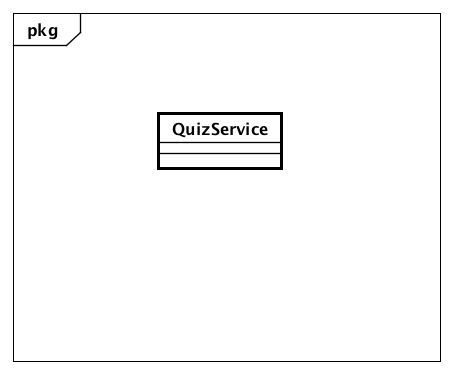
\includegraphics[scale=0.45]{UML/Classi/Front-End/QuizziPedia_Front-end_Services_ QuizService.png}
	\caption{QuizziPedia::Front-End::Services::QuizService}
\end{figure}
\begin{itemize}
	\item \textbf{Descrizione}: questa classe permette di ottenere i dati di un quiz tramite delle parole chiave inserite dall'utente nella barra di ricerca;
	\item \textbf{Utilizzo}: fornisce le funzionalità per ottenere i dati di un quiz in seguito ad una ricerca dell'utente, passando i risultati ai controllers. Ritorna dei riferimenti alle domande del quiz;
	\item \textbf{Relazione con altre classi:}
	\begin{itemize}
		\item \textit{IN} \texttt{SearchController} 
		\item \textit{IN} \texttt{QuestionsController}
		\item \textit{IN} \texttt{QuestionnaireDetailsController} 
		\item \textit{IN} \texttt{FillingQuestionnaireController} 
		\item \textit{OUT} \texttt{TemplateQuestionnaireController} 
		\item \textit{OUT} \texttt{RegistrationManagementController} 
		\item \textit{OUT} \texttt{ResultsController} 
		\item \textit{OUT} \texttt{QuestionnaireManagementController} 
		
	\end{itemize}
	\item \textbf{Attributi:}
	\begin{itemize}
		\item 
	\end{itemize}
	\item \textbf{Metodi:}
	\begin{itemize}
		\item 
	\end{itemize}
\end{itemize}

\paragraph{QuizziPedia::Front-End::Services::ErrorService}
\begin{figure}
	\centering
	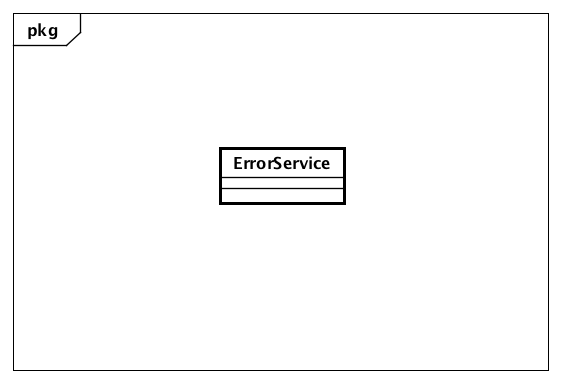
\includegraphics[scale=0.45]{UML/Classi/Front-End/QuizziPedia_Front-end_Services_ ErrorService.png}
	\caption{QuizziPedia::Front-End::Services::ErrorService}
\end{figure}
\begin{itemize}
	\item \textbf{Descrizione}: questa classe permette di gestire il recupero e la gestione dei messaggi di errore;
	\item \textbf{Utilizzo}: fornisce al controller i giusti messaggi di errore da mostrare all'utente;
	\item \textbf{Relazione con altre classi:}
	\begin{itemize}
		\item \textit{IN} \texttt{ErrorController} 
	\end{itemize}
	\item \textbf{Attributi:}
	\begin{itemize}
		\item 
	\end{itemize}
	\item \textbf{Metodi:}
	\begin{itemize}
		\item 
	\end{itemize}
\end{itemize}

\paragraph{QuizziPedia::Front-End::Services::StatisticsService}
\begin{figure}
	\centering
	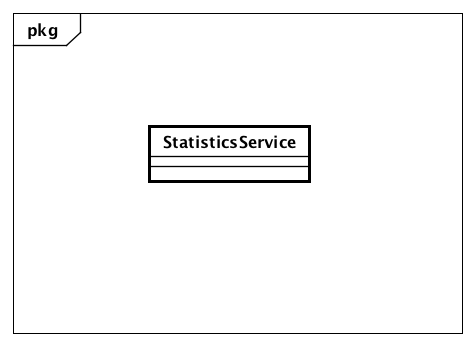
\includegraphics[scale=0.45]{UML/Classi/Front-End/QuizziPedia_Front-end_Services_ StatisticsService.png}
	\caption{QuizziPedia::Front-End::Services::StatisticsService}
\end{figure}
\begin{itemize}
	\item \textbf{Descrizione}: questa classe permette di ottenere le statistiche dell'utente;
	\item \textbf{Utilizzo}: fornisce al controller le statistiche salvate;
	\item \textbf{Relazione con altre classi:}
	\begin{itemize}
		\item \textit{IN} \texttt{StatisticsController} 
	\end{itemize}
	\item \textbf{Attributi:}
	\begin{itemize}
		\item 
	\end{itemize}
	\item \textbf{Metodi:}
	\begin{itemize}
		\item 
	\end{itemize}
\end{itemize}

\paragraph{QuizziPedia::Front-End::Services::QuestionServices}
\begin{figure}
	\centering
	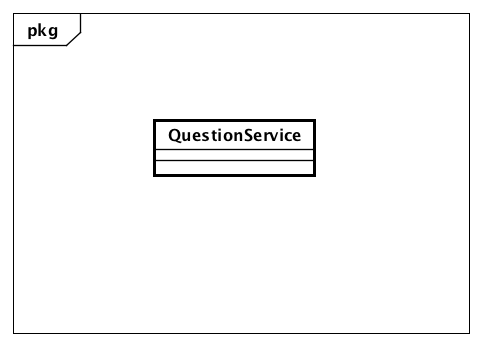
\includegraphics[scale=0.45]{UML/Classi/Front-End/QuizziPedia_Front-end_Services_ QuestionService.png}
	\caption{QuizziPedia::Front-End::Services::QuestionService}
\end{figure}
\begin{itemize}
	\item \textbf{Descrizione}: questa classe permette di ottenere domande esistenti e salvare nuove domande;
	\item \textbf{Utilizzo}: utilizzata per richiedere domande presenti nel database. Offre inoltre delle funzionalità per inserire nuove domande;
	\item \textbf{Relazione con altre classi:}
	\begin{itemize}
		\item \textit{IN} \texttt{TrueFalseController} 
		\item \textit{IN} \texttt{MultiplyQuestionsController} 
		\item \textit{IN} \texttt{ConnectionQuestionsController} 
		\item \textit{IN} \texttt{ImagesSortingQuestionsController} 
		\item \textit{IN} \texttt{StringsSortingQuestionsController} 
		\item \textit{IN} \texttt{FillingQuestionsController} 
		\item \textit{IN} \texttt{ClickableAreaQuestionsController} 
		\item \textit{IN} \texttt{EditorQMLController} 
		\item \textit{IN} \texttt{QuestionsManagementController} 
		\item \textit{IN} \texttt{KeywordsController} 
		\item \textit{IN} \texttt{QuestionnaireQuestionsManagementController} 
		
	\end{itemize}
	\item \textbf{Attributi:}
	\begin{itemize}
		\item 
	\end{itemize}
	\item \textbf{Metodi:}
	\begin{itemize}
		\item 
	\end{itemize}
\end{itemize}

\paragraph{QuizziPedia::Front-End::Services::UserDetailsService}
\begin{figure}
	\centering
	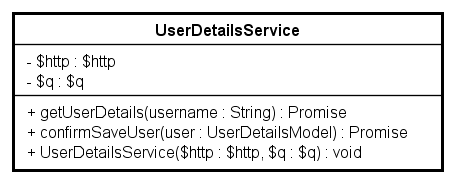
\includegraphics[scale=0.45]{UML/Classi/Front-End/QuizziPedia_Front-end_Services_UserDetailsService.png}
	\caption{QuizziPedia::Front-End::Services::UserDetailsService}
\end{figure}
\begin{itemize}
	\item \textbf{Descrizione}: questa classe permette di ottenere i dati personali degli utenti;
	\item \textbf{Utilizzo}: utilizzata per ottenere i dati personali di un utente. Permette inoltre di trovare i dati di utenti ricercati tramite l'apposita barra di ricerca;
	\item \textbf{Relazione con altre classi:}
	\begin{itemize}
		\item \textit{IN} \texttt{SearchController} 
		\item \textit{OUT} \texttt{UserDetailsController} 
		\item \textit{OUT} \texttt{ProfileManagementController} 
	\end{itemize}
	\item \textbf{Attributi:}
	\begin{itemize}
		\item 
	\end{itemize}
	\item \textbf{Metodi:}
	\begin{itemize}
		\item 
	\end{itemize}
\end{itemize}
